\documentclass[journal,twocolumn,letterpaper,12pt]{article}
\usepackage{colortbl}
\usepackage{graphicx}
\usepackage{geometry}
\usepackage{float}
\usepackage[table,xcdraw]{xcolor}
\usepackage{amssymb}
\usepackage{amsmath}
% Cite URL and break line
\usepackage{url}
\usepackage{breakurl}
\def\UrlBreaks{\do\/\do-}
%%
\usepackage{setspace}
\usepackage{slashbox}
\usepackage{flushend,cuted}
\usepackage{makecell,rotating,multirow,diagbox}
\usepackage{listings}
\usepackage[framed,numbered,autolinebreaks,useliterate]{mcode}
\geometry{a4paper,margin=15mm,bindingoffset=15mm,heightrounded,}
\renewcommand\thesection{\Roman{section}}
\tolerance=5
\emergencystretch=\maxdimen
\hyphenpenalty=0
\hbadness=10
\definecolor{mygray}{gray}{0.8}
%\setlength{\intextsep}{10mm}
%\setlength{\belowcaptionskip}{5mm}
% define the title
\author{\textsl{Zhikun Zhu; ID:~29356822}}
\title{Machine Learning Coursework One}
\setlength{\parindent}{0pt}
\begin{document}
% generates the title
\maketitle
% insert the table of contents
%\tableofcontents
\section{Introduction}
There are two parts in this coursework, \textsl{Neural Network Approximation} and \textsl{Time Series Prediction}. Firstly, we will discuss the two-class pattern classification problem. Decision boundary for both Bayesian and feedforward neural network methods will be plotted and their performance will be discussed. Then, we will use a feefforward network and linear regression method to predict chaotic time series and financial time series.\\

\section{NN Approximation}
In this part, we are given two classes of data $X_1$ and $X_2$ that follow multivariate Gaussian distributions with distinct mean and covariance. These two classes will classifed by Bayesian classifier and Feedforward Neural Network (FNN) resectively, and both performance will be discussed.

\subsection{Bayesian Classifier}
According to Bayesian theorem, the posterior probability can be calculated from prior probability:
\begin{equation}
  ~P[w_j|X] = \frac{~p[X|w_j]~P[w_j]}{\sum_{i=1}^K~p[X|w_i]~P[w_i]}
\end{equation}
The denominator is a constant ($P[X]$). In order to maximize posterior probability, we need assign $x$ to the class which has the highest probability to generate $x$, which means to optimize $p[X|w_j]$.\\
Therefore, it should be straightforward that for a 2-class pattern classification problem we assign $X$ to $w_j$ if $P[w_j|X]>0.5$. Then the Bayesian optimal boundary is:
\begin{equation}
  ~P[w_1|X] = ~P[w_2|X] = 0.5
\end{equation}
Substitute the expression of Bivariate Gaussian Distributions into Equation.2, and since we equally drawn 100 samples from $X_1$ and $X_2$ to generate the training sets, which means $p[w_1]=p[w_2]=0.5$. Then, Equation.2 becomes:
\begin{displaymath}
  \begin{array}{c}
    \frac{1}{(2\pi)^{p/2}det(C_1)^{1/2}}exp{\{\frac{1}{2}(x-m_1)^TC_1^{-1}(x-m_1)}\} \\
    \quad \\
    =\frac{1}{(2\pi)^{p/2}det(C_2)^{1/2}}exp{\{\frac{1}{2}(x-m_2)^TC_2^{-1}(x-m_2)}\}
  \end{array}
\end{displaymath}
Take $log(\cdot)$ on both side, and notice that covariance matrixes $C_1$ and $C_2$ are positive semidefinite and symmetric, which means $C_i = C_i^{T}$. Since the detailed derivative process are already done in LAB 3, then I samply write the answer of the reduced expression bolow:
\begin{equation}
  x^T(C_1^{-1}-C_2^{-1})x + 2w^Tx + b = log_e(\frac{|C_2|}{|C_1|})
\end{equation}
Where $b = (m_1^TC_1^{-1}m_1 - m_2^TC_2^{-1}m_2)$ and $w=(m_2^TC_2^{-1}-m_1^TC_1^{-1})$.\\

\begin{figure}[H]
\centering
   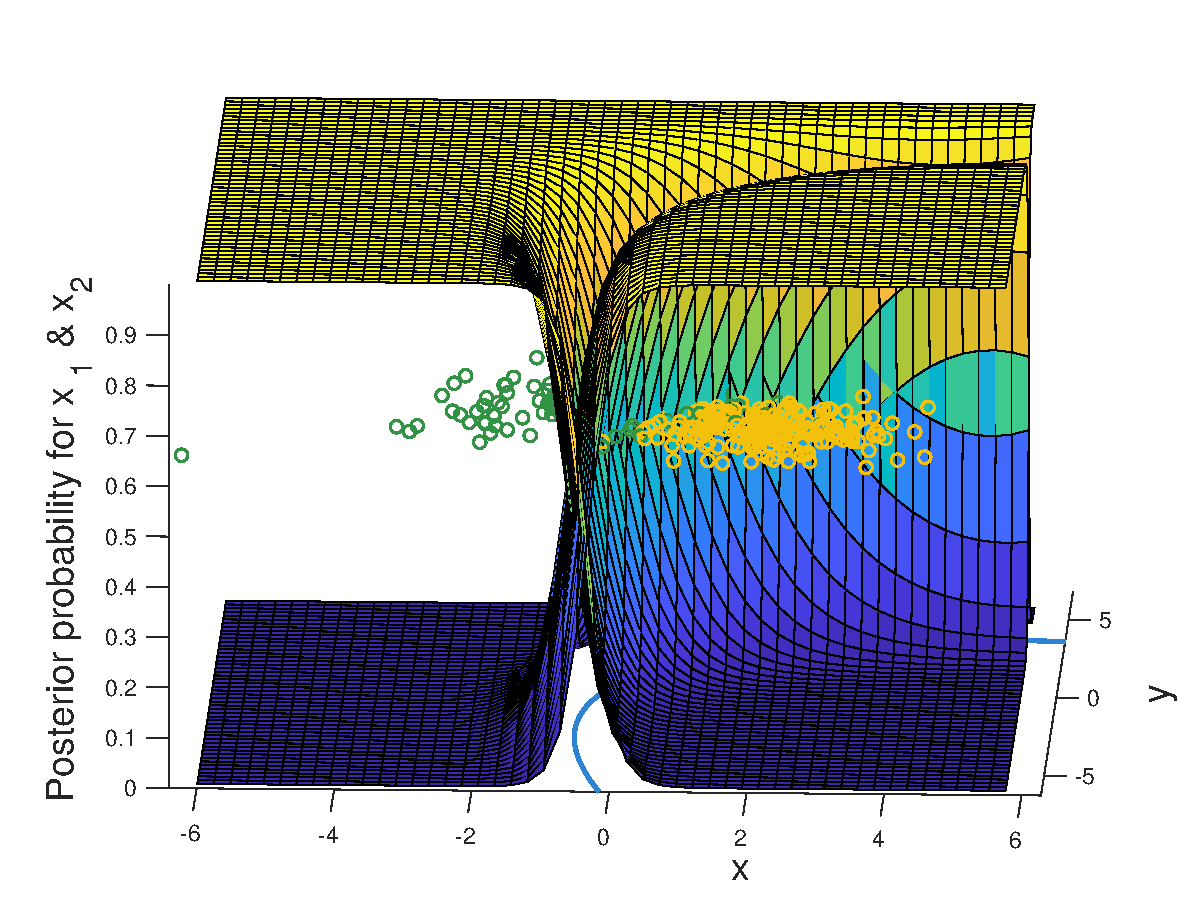
\includegraphics[width=0.5\textwidth]{PP.eps}

    \textsl{\caption{Posterior Probability Graph}}
\end{figure}
Figure.1 shows posterior probabilities for both $P[w_1|X]$ and $P[w_2|X]$. Besides, the samples drawn from $X_1$ (red) and $X_2$ (green) are also plotted in the 3D graph, their z-axis' value are set to 0.5, putting them to the decision plane where $~P[w_1|X] = ~P[w_2|X]=0.5$. The Bayesian optimal boundary was also projected to x-y plane.\\
Figure.2 shows 200 samples equally drawn from $X_1$ and $X_2$. The bayesian optimal boundary sort the point to the class with highest posterior probability. Nevertheless, it still sorts some data in the wrong classes, which can be explained by the fact that the data is more likely be generated by $X_1$, whereas, the small probability event happens (it was generated by $X_2$).\\
\begin{figure}[htbp]
\centering
   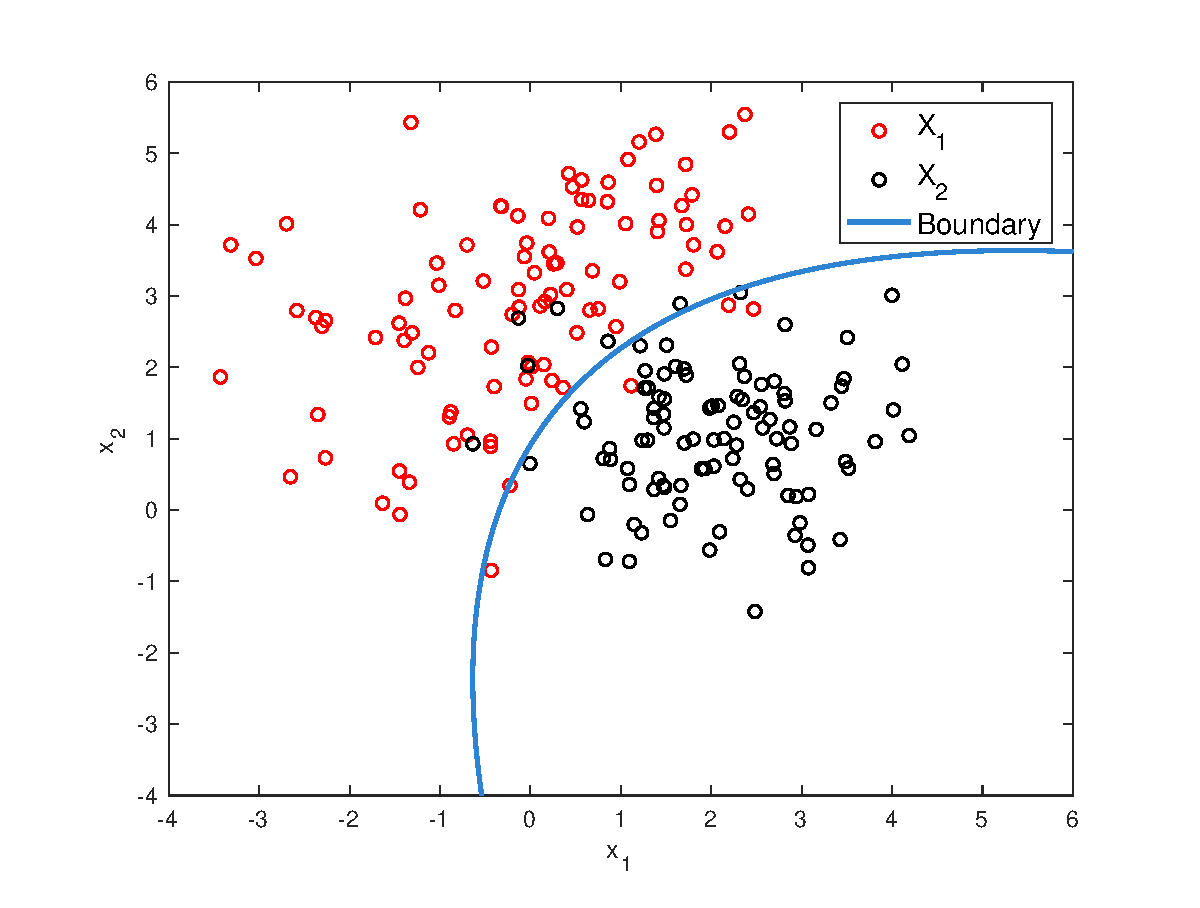
\includegraphics[width=0.4\textwidth]{BayesianB.eps}

    \textsl{\caption{Bayesian Optimal Boundary}}
\end{figure}
\subsection{Feedforward NN}
A FNN with 20 hidden neurons is trained by 200 samples drawn from $X_1$ (Tag: 1) and $X_2$ (Tag: -1). Then the original training set and a new test set (200 samples equally generated by $X_1$ and $X_2$) are used to test the performance of the neural network. The error rate is shown in Table.1. The error is the average error of 40 test sets in order to avoid occasionality.
\begin{table}[htbp]\footnotesize
  \begin{center}
    \begin{tabular}{|c|c|c|c|}
      \hline
      Method & \begin{tabular}[c]{@{}l@{}}Bayesian\\ Boundary\end{tabular} & \begin{tabular}[c]{@{}l@{}}NN with\\ Training Set\end{tabular} & \begin{tabular}[c]{@{}l@{}}NN with\\ Test Set\end{tabular} \\ \hline
      Error  & 0.0701                                                      & \cellcolor[HTML]{C0C0C0}{0.0694}          & 0.0870                                                     \\ \hline
    \end{tabular}
  \end{center}
\caption{\textsl{Error rate comparison}}
\end{table}
\\
According to Table.1, we can find that the minimum error rate is from the FNN with training set as input. However, when it comes to the test set, the performance of Bayesian boundary surpass feedforward NN, since bayesian optimal boundary is optimized by probability. FNN's bad performance in test set is caused by overfitting, which will be discussed in later section.\\
One specific classification result generated by FNN with training set is shown in Figure.3, which error rate is $7.5\%$.\\
The data points denoted by `o' are correctly classified and `x' denotes misclassified data. And the red points are recognised belong to $X_1$ and black points belong to $X_2$.
\begin{figure}[htbp]
  \centering
   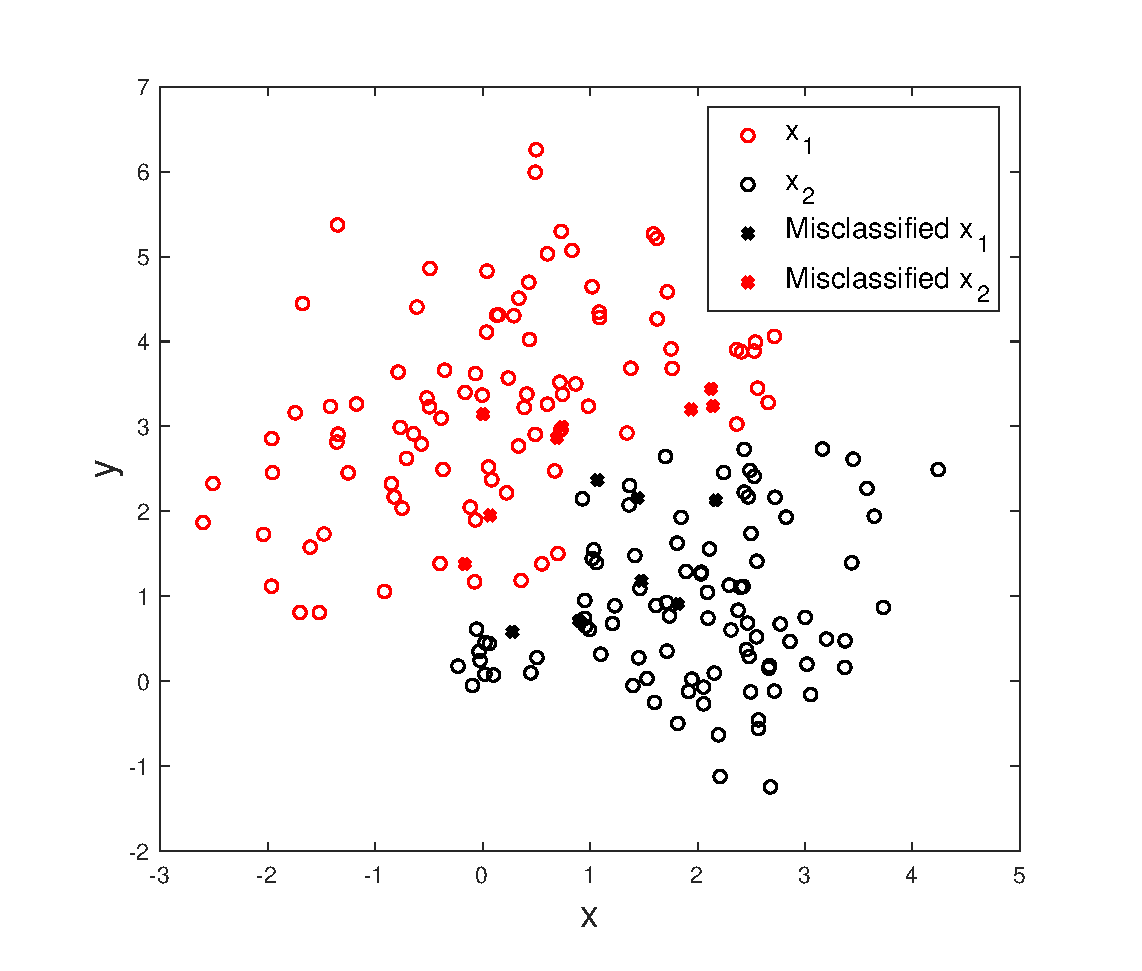
\includegraphics[width=0.5\textwidth]{FNNT.eps}

    \textsl{\caption{Classification results of forward NN.}}

\end{figure}
\\
The class boundary of FNN is plotted in Figure.4, which is generated by training the square area
$ (x,y) \in
\left\{
  \begin{array}{ccc}
    |x|\leq 5\\
    |y|\leq 5\\
  \end{array}
\right.$
with a step equals to 0.2. The red points are area which will be classifed as $X_1$ and black for $X_2$.\\
Since I choose to tag $X_1$ by `1' and $X_2$ by `-1', the final decision boundary should be $1-1 = 0$, which can also be verified by the colour boundary between red (recognised belong to $X_1$) and black (recognised belong to $X_2$) in Figure.4.
\begin{figure}[htbp]
\centering
   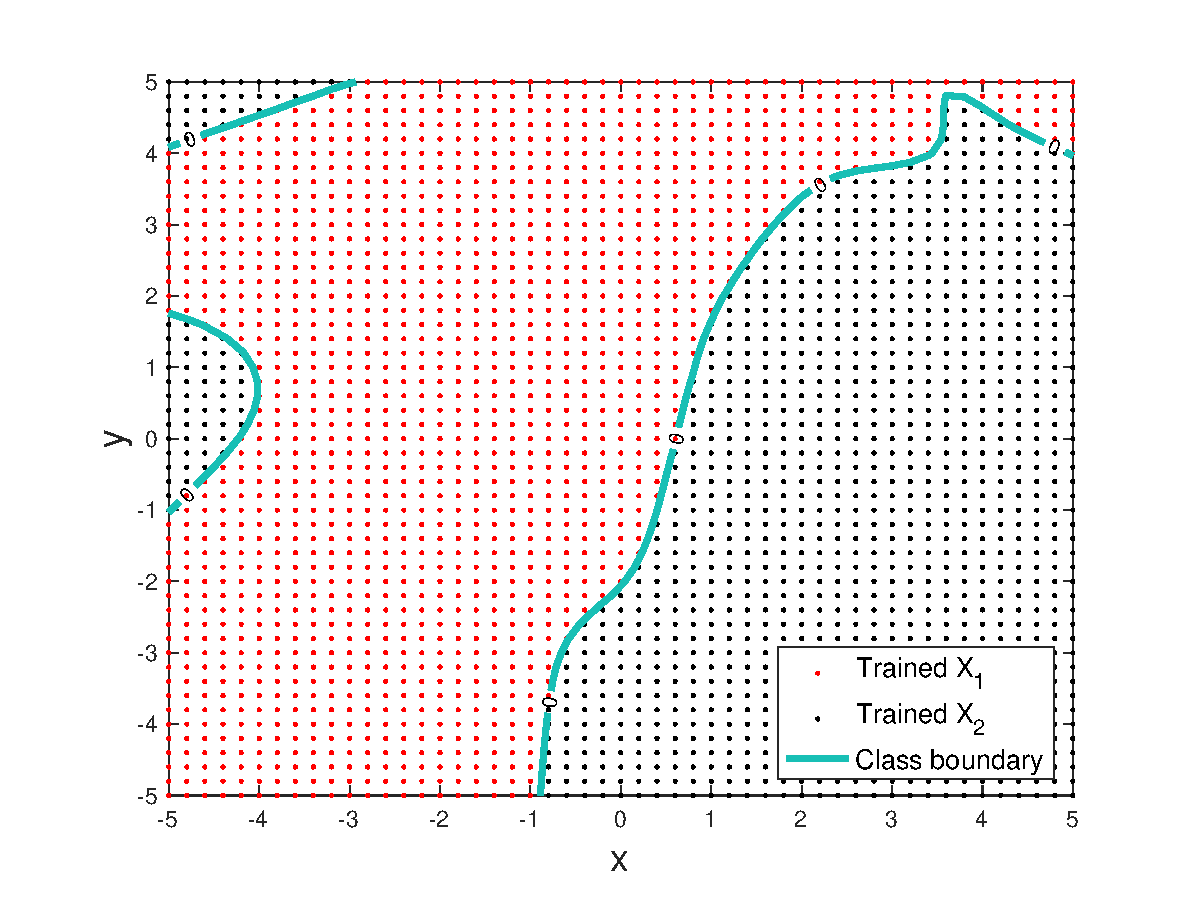
\includegraphics[width=0.5\textwidth]{CBFNN.eps}
    \textsl{\caption{Class boundary of forward NN.}}

\end{figure}
\\
In order to compare the performance between FNN with different hidden neurons size and Bayesian optimal boundary, I trained several neural networks with hidden layer size varying from 10 to 55 with a step equals to 5. The size of training set was set to 20,000 in order to minimize occasionality. Once the networks are trained, they are used to process 40 test sets with 2000 samples equally drawn from $X_1$ and $X_2$. The final error rate is got by taking average among the error rates of all test sets, which is shown in Figure.5.
\begin{figure}[htbp]
\centering
   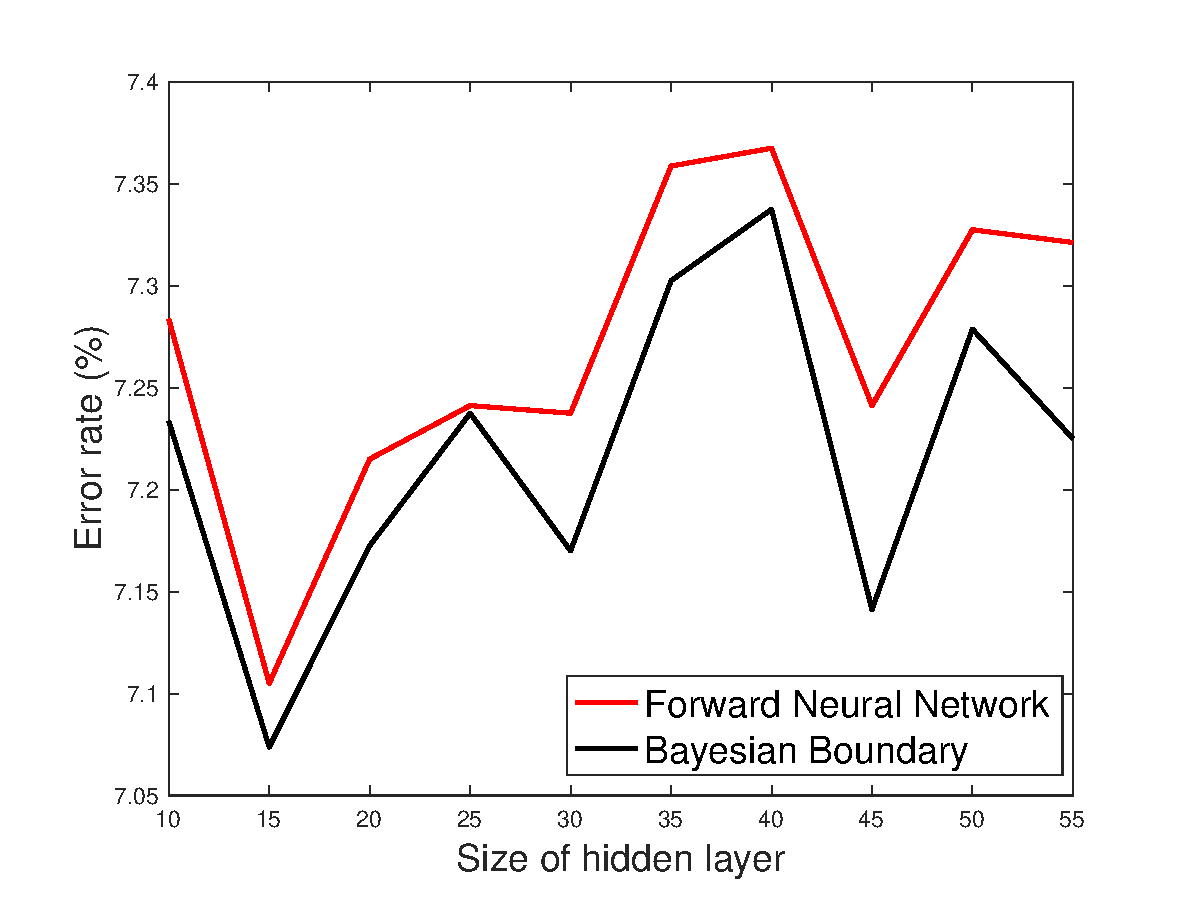
\includegraphics[width=0.4\textwidth]{NNBB.eps}
    \textsl{\caption{Error rate comparison betwenn forward NN and Bayesian boundary.}}
\end{figure}
\\
It is clear that the performance of FNN is a bit worse than the Bayesian boundary, which error rate can be considered as the lower boundary of the neural networks' error rate.\\
Besides, the difference between two error rates (Bayesian \& FNN) as well as FNN's error rate are not getting smaller as the increase of the hidden neurons.
\section{Time \qquad Series \\ Prediction}
There are two parts in this section, the former one is to train a FNN using Mackey-Glass chaotic time series \cite{mackey1977oscillation} generated by \cite{MackeyGlass} to predict the value at time t using previous 20 time slots. The FNN will work in two mode, one step ahead and free running, respectively. And its performance will be compared with linear regression method.\\
Then we will train a FNN with same structure as previous one to predict the future FTSE 100 index \cite{investing.com} utilizing existing data like previous close price and Volume Traded, highest price, etc.
\subsection{Data Normalization}
The reason behind data normalization \cite{ioffe2015batch} is that, for a p-demension input data set (training set), each demension have different means and variances, which will significantly influence the weights $w_i$ of linear regression or neural network. Besides, it will slow the training speed since for a gradient descent method, the direction of gradient descent is pointing to the tangential direction. Figure below shows the descent direction under case with and without normalization.
\begin{figure}[htbp]
\centering
   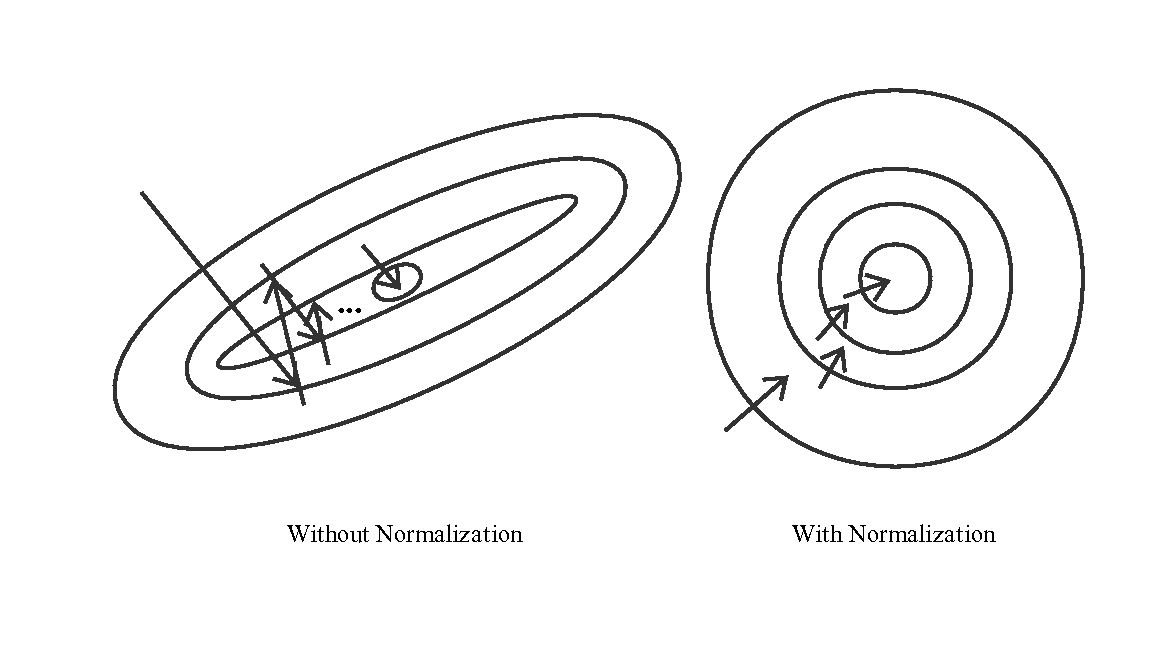
\includegraphics[width=0.5\textwidth]{Normal.pdf}
    \textsl{\caption{Descent direction without normalization (Left) v.s. with normalization (Right).}}
\end{figure}
\\
For example, according to Lab 4, we use 13 parametres to predict the house price in Boston. Each of the 13 parametres have distinct means and variances, normalization will boost the algorithm's efficiency. Futhermore, we also utilize $L_1$ norm to get the sparse solution of $w$ in linear regression, if we use the training set without normalization, the results of sparse solution will be greatly influenced by the demensions with large means.\\
According to the requirement, we will use 20 previous time slots to predict the 21st time slot's value, then, we have a training set with 20 demensions having similar mean and variance. Then, normalization will only have limitted influence on the training results. Then, I only normalized each demension with respective means and tried to preserve the their variances.
\subsection{Chaotic Time Series}
Firstly,a Mackey-Glass chaotic time series with N=2000 samples were generated, which is plotted in Figure.6 (black). The specification asks to use the first $N = 1500$ data as training set and remaining 500 data as test set, and use previous $p = 20$ time slots to predict the next time slot's value. Then we need to generate a  $(N-p) \times p$ training matrix $X_{Tr}$, which is shown in Table.2.
\begin{table}[H]\footnotesize
  \begin{center}
    \begin{tabular}{|c|c|c|c|c|}
      \hline
      \backslashbox{\textbf{Row}}{\textbf{Col}}    & 1       & 2       & ... & 20      \\ \hline
      1    & x(1)    & x(2)    & ... & x(20)   \\ \hline
      2    & x(2)    & x(3)    & ... & x(21)   \\ \hline
      ...  & ...     & ...     & ... & ...     \\ \hline
      1480 & x(1480) & x(1481) & ... & x(1499) \\ \hline
    \end{tabular}
  \end{center}
  \textsl{\caption{FNN Training set.}}
\end{table}
And the target $y$ of the training matrix is:
\begin{displaymath}
  y=[x(21),x(22),...,x(1500)]^T
\end{displaymath}
 The prediction results (Training \& Test set)of linear regression method is shown in Figure.7, as well as the original input.
\begin{figure}[H]
  \centering
   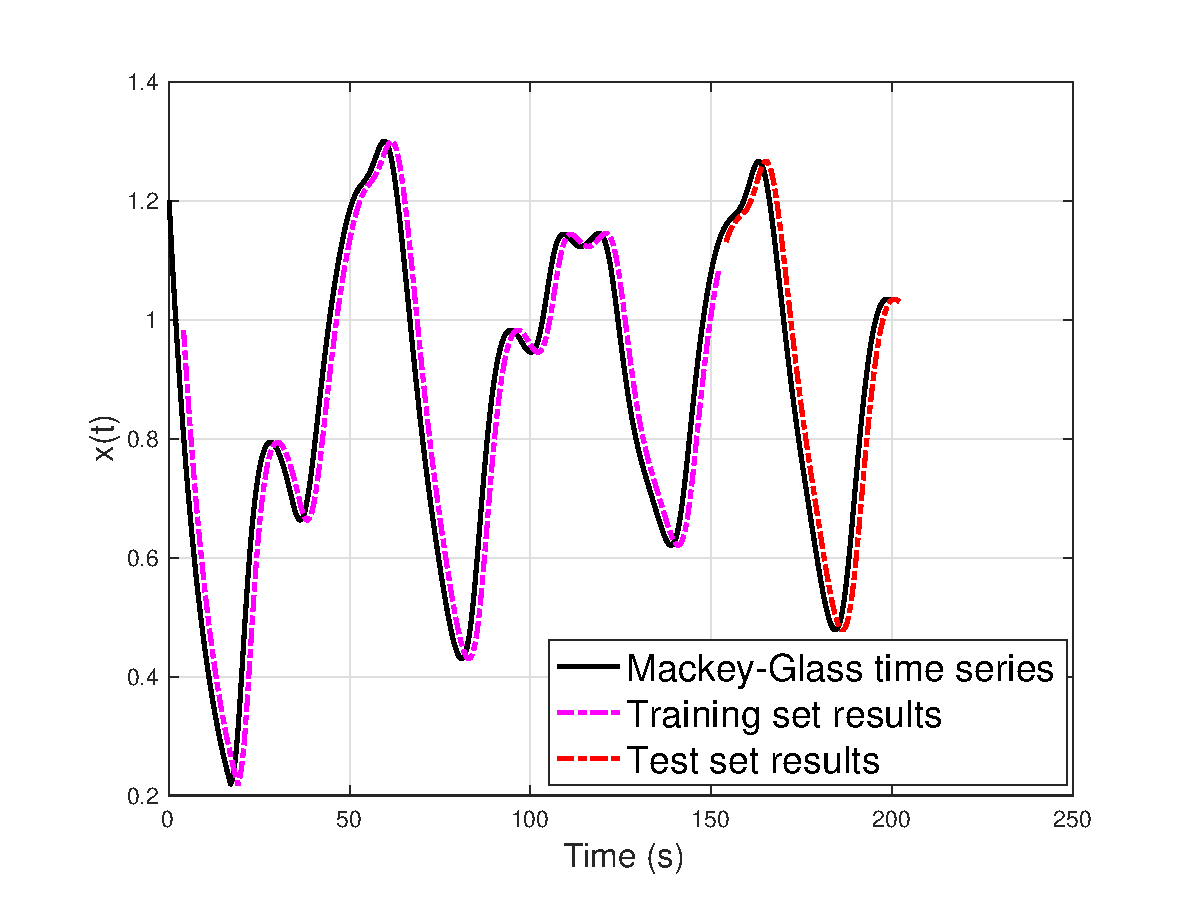
\includegraphics[width=0.5\textwidth]{MKTS.eps}
    \textsl{\caption{Training results with linear regression method. (Both training and test results is delayed with 2 seconds for the convenience of viewing.)}}
\end{figure}
The error, which got by taking $L_2$ norm of $X_{Real}(t)-X_{Predicted}(t)$ and normalized by length of the set, for training and test set are $ 2.4638\cdot10^{-6}$ and $6.5027\cdot10^{-7}$, respectively.\\
The feedforward neural network is trained by $X_{Tr}^T$ and $y^T$, and it is used to predict the time series using $X_{Tr}^T$ and test matrix $X_{Te}^T$, which is generaed same with $X_{Tr}$.\\
The prediction results of the FNN under free running mode is shown in Figure.7, which means the FNN use the first 20 data of the Mackey-Glass time series to predict 21st data and use the 21st data and previous 19 data to predict the 22nd data, so on and so forth.
\begin{figure}[htbp]
  \centering
   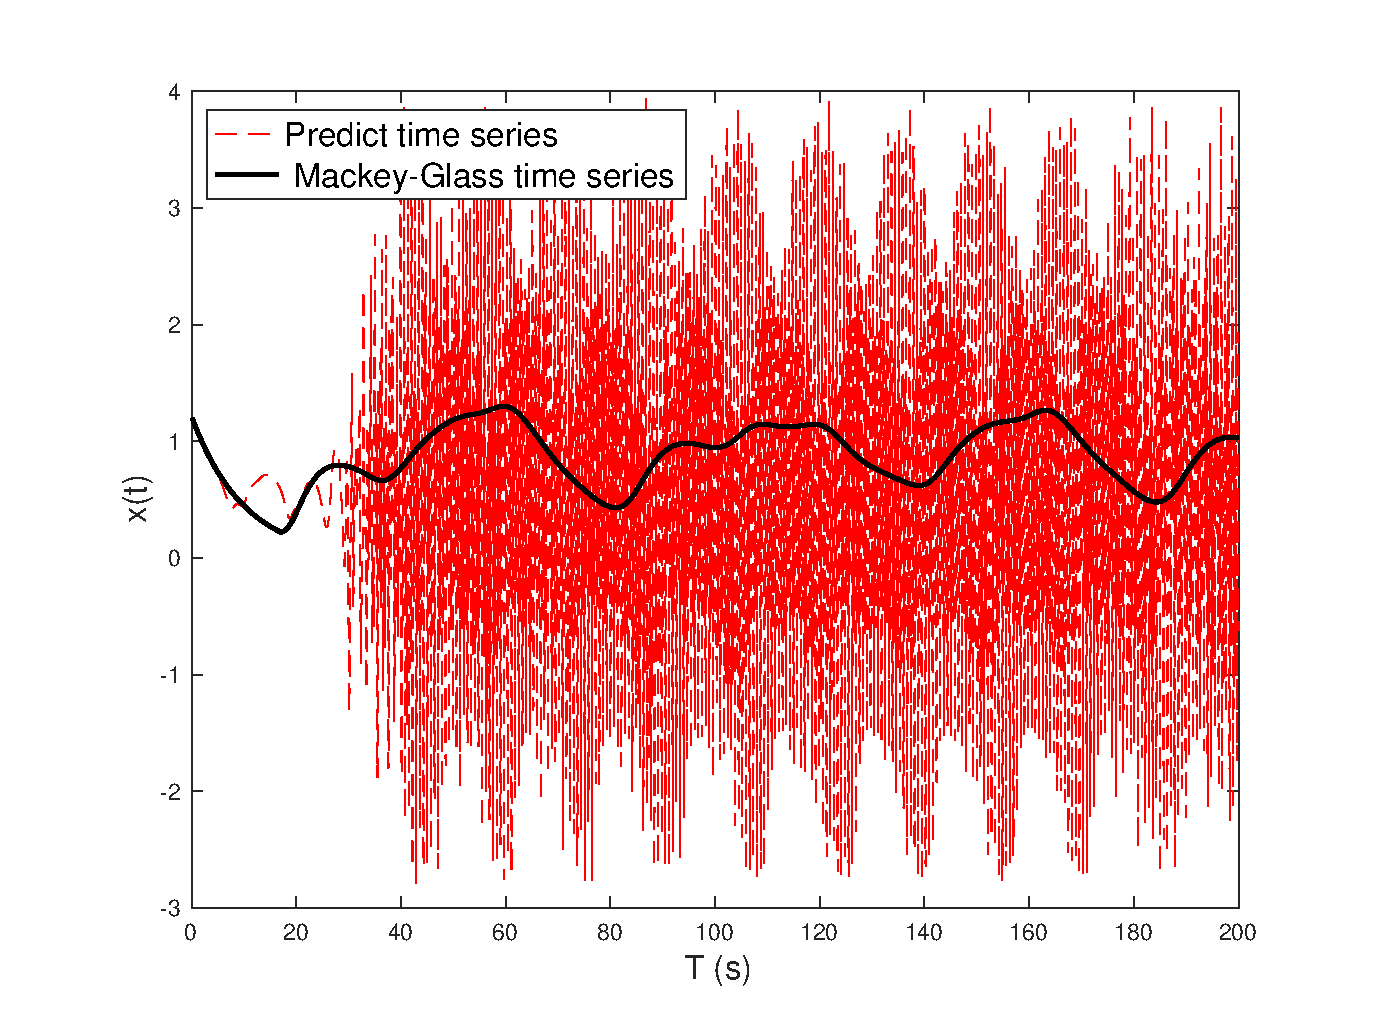
\includegraphics[width=0.5\textwidth]{FNNFR.eps}
    \textsl{\caption{FNN prediction results under free running mode.}}
\end{figure}
\\
According to Figure.8, the accuracy of the prediction only  sustained for a few seconds. However, the predicted data also sustained oscillations. \\
I tried to change the $\delta$ that used to generate Mackey-Glass series and test the prediction results under free running mode. By observaing Figure.7 \& 8, the begining part of the series is transient to the overall time series. Since the algorithm is running under free running mode, then the first 20 data is of vital importance to the future prediction, then the begining part is removed in the algorithm and the results is shown in Figure.9.
\begin{figure}[htbp]
  \centering
   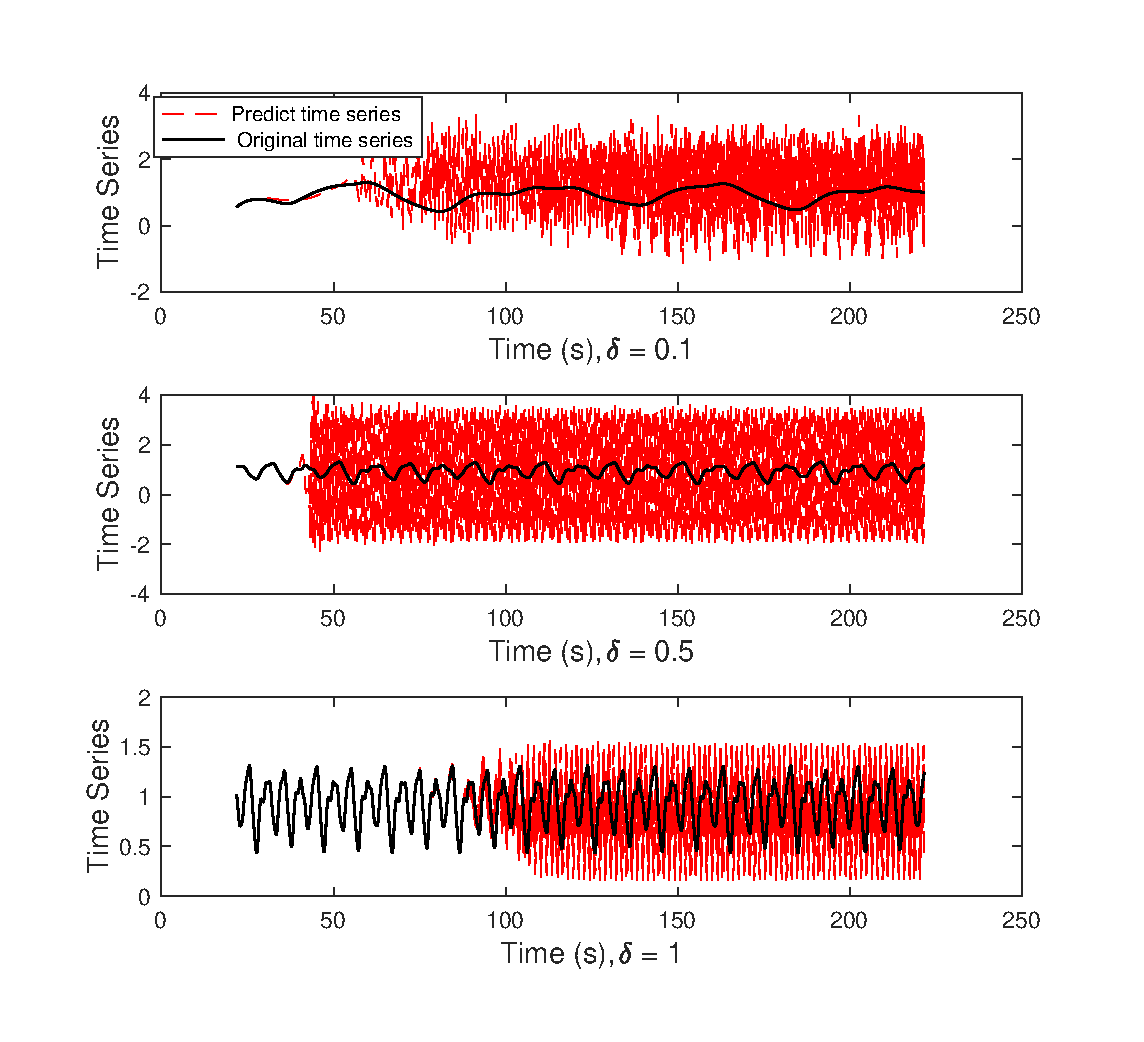
\includegraphics[width=0.5\textwidth]{freeDiffDelta.eps}
    \textsl{\caption{ Prediction results under free running mode varying from different $\delta$. }}
\end{figure}
\subsection{Financial Time Series}
In this section FEST 100 historical data of past 5 years will be used to train the FNN. Firstly, We will continue to use previous 20 days' close price to predict 21st day's close price. The results is shown in Figure.8.
\begin{figure}[htbp]
  \centering
   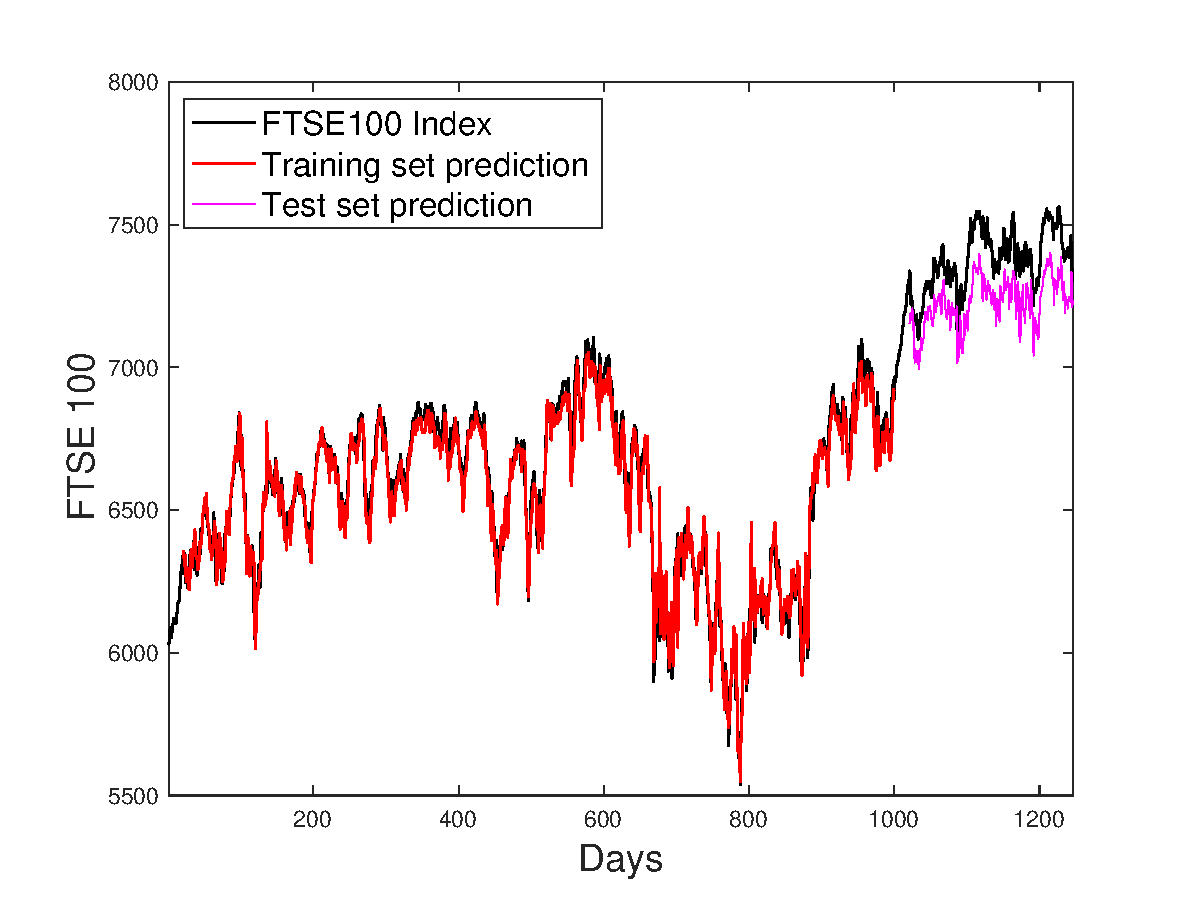
\includegraphics[width=0.5\textwidth]{FTSE100.eps}
    \textsl{\caption{FTSE100 predicted close price vs. real close price. }}
\end{figure}
\\
The error which is calculate by taking $L_2$ norm between predicted price and real price is $ 2.1176\times10^3$ for training set and $ 2.5304\times10^3$  for test set. Since the error may be affected by the length of input size, we  can normalize the error by:\\
\begin{equation}
  Error = \frac{\sqrt{\sum_{i=1}^{N}x_P(i)^2-x_O(i)^2}}{N}
\end{equation}
Where $x_P(t)$ denotes the predicted sequence, $x_O(t)$ is the real sequence, and $N$ is the length of the sequence.
We got 1246 days' FTSE 100 index, and 1000 out of them were used to train the network and remains are used to test it. Then, the size of training set is $980\times20$, and $226\times20$ for the test set. Finally, the normalized error are $ 2.1608$ and $  11.1966$ for training set and test set, respectively.\\
We can also train the FNN using close price and volume of trade simultaneously, which are expected to have better prediction performance. The error which calculated by Equation.3 for training set and test set is 1.7772 and 16.7640, respectively.\\
\begin{figure}[htbp]
  \centering
   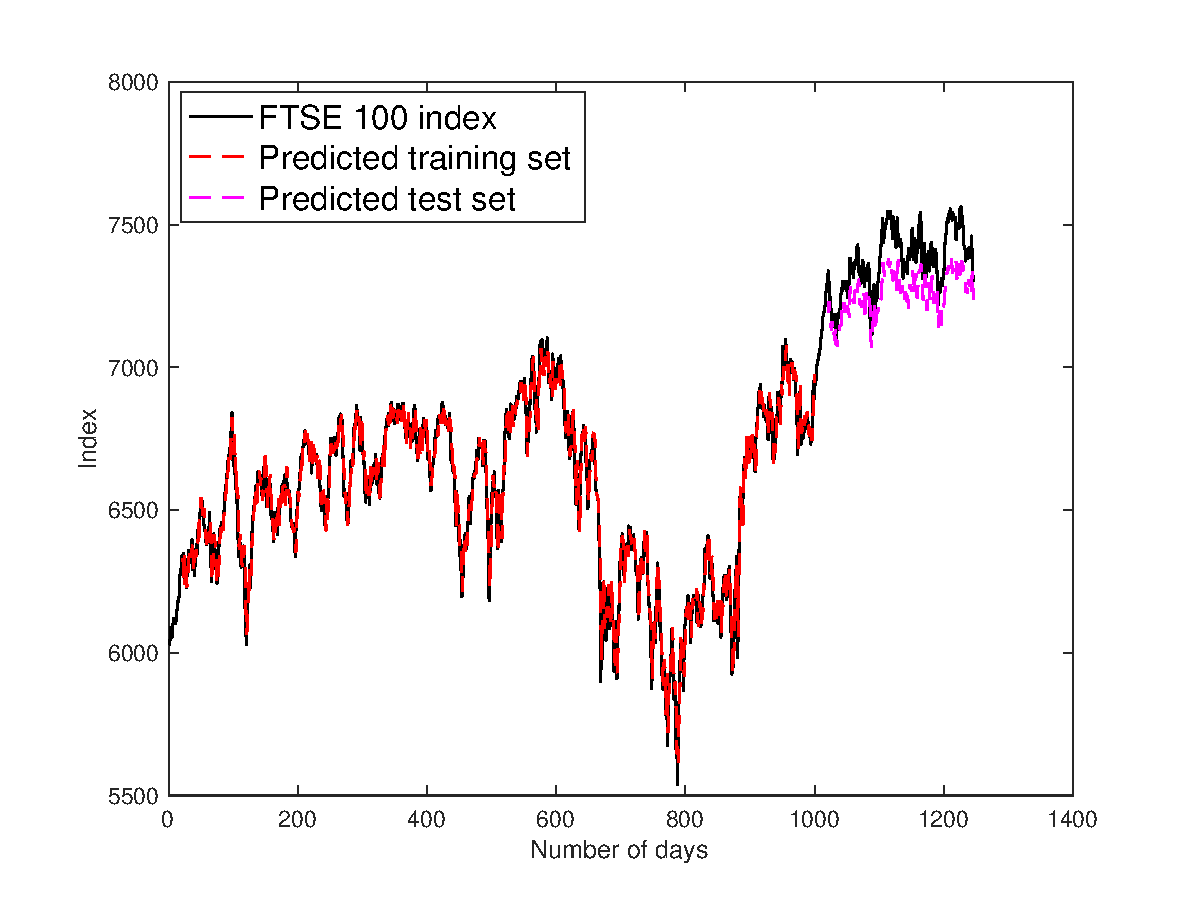
\includegraphics[width=0.5\textwidth]{FTSE2.eps}
    \textsl{\caption{FTSE100 prediction results by FNN using close price \& volume of trade. }}
\end{figure}\\
In comparison of different parametres' influences on the prediction accuracy of FNN, I generated new training sets using close price combine with other five parametres separately, which are : 1. Open Price; 2. Higest Price; 3. Lowest Price; 4. Volumn traded; 5. Change (\%). \\
These five training sets are used to train FNN with hidden neurons varying from 10 to 35 in a step equals to 5. Then all FNNs are used to predict the FTSE 100 index using test sets for 20 times in case for occasionality. The final predction error per sample calculated by Equation.3 is shown in Figure.10.
\begin{figure}[htbp]
  \centering
   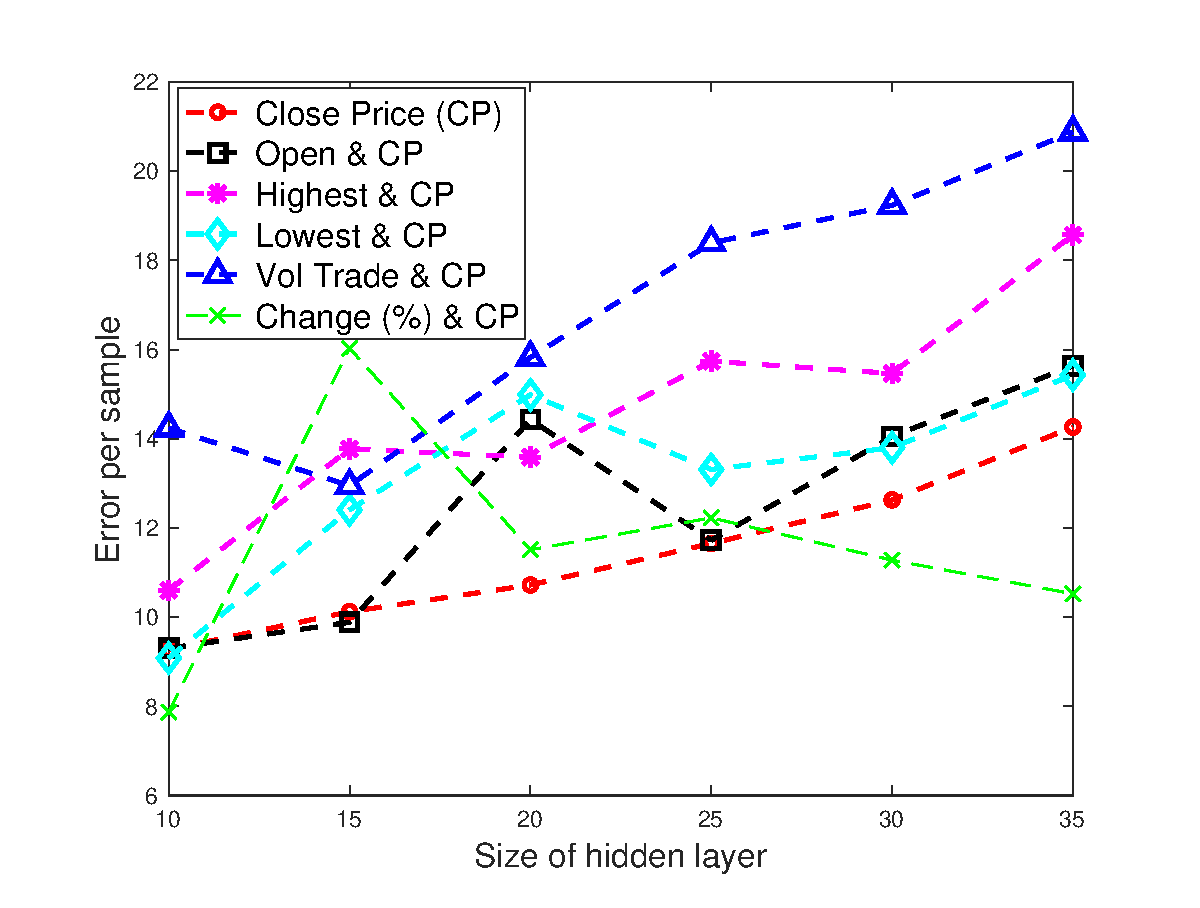
\includegraphics[width=0.5\textwidth]{changeAsSizePara.eps}
    \textsl{\caption{FTSE100 prediction error (Test Set) varying from different parametres used to train the neural network ans size of hidden layer size.}}
\end{figure}
\\
According to Figure.10, there is no evidence show that the error per sample trend to decrease as the increase of hidden layer size, whereas it shows a increasing trends, which may be caused by overfitting. In Lab 4, we use $L_1$ norm of $w$ as a constraint to avoid overfitting. To solve such problem in single-hidden-layer feedforward networks (SLFNs), \cite{feng2009error} proposed a structure called Extreme Learning Machine (ELM) to determine the size of hidden layer to avoid overfitting and minimize error.\\
Besides, the prediction results suggest that the neural network that trained only by the close price has the minimum error, which is also large for test set. One way to improve its performance is to use ELM method to suppress overfitting. Another way is to update the FNN by latest data, which means we move down the window of training set every day.\\
According to Figure 10 \& 11, the error of test set is large, and its prediction in the short time is inaccurate, whereas, its prediction tendency in the long time scale is basically follow the read index. Then, the prediction results can be used as a reference but cannot make money directly.
\section{Conclusion}
In this coursework, firstly, the expression of Bayesian optimal boundary were briefly drived. Then, the performance between Bayesian classification and feedforward neural network (with different size of hidden layer) were compared, where I believe the error of Bayesian optimal boundary is the lower limit of FNN.\\
In time series prediction, the motivation behind data normalization of each dimension is discussed. Both linear regression and feedforward neural network were used to predict the Mackey-Glass time series and their performance is discussed. Furthermore, they were also used to perform prediction under free running mode.\\
In the part of financial time series prediction, the FNN's performance on test set is evidently worse than training set. Besides, the training method which combine the close price and volumn traded together isn't improved the performance.\\
Nevertheless, training the FNN using close price only seems to have the best performance than combine any two of the parametres together. Future analysis may consider combine three or more parametres together and employ ELM method to see if the performance is improved.

\bibliographystyle{ieeetr}
\bibliography{cite}
\end{document}
